
In 1997, Deep Blue, a supercomputer built by IBM, won a six games match against Garry Kasparov, the current world chess champion. Humans got beaten in Chess, but remain undefeated in other games. Consequently, researchers are looking for improvements in Artificial Intelligence.
\newline

The project is called \emph{Fast \& Furious Game Playing, Monte Carlo Drift}. Its purpose is to create an Artificial Intelligence able to compete against humans using the \emph{Monte Carlo Tree Search}.
\newline

The focus of this project is on two player strategy board games, while avoiding games already solved\footnote{A game solved is a game where good algorithms are able to find the perfect move in each situation to win, or to draw. For instance, \textit{Tic Tac Toe} or \textit{Draughts} are solved games.}. That is why this project is about tha game \emph{Arimaa}.
\newline

To evaluate the best move, the algorithm develops a tree by creating nodes for of all possible moves. Then it computes statistics by evaluating these nodes. These statistics can be the result of a deeper exploration of a node, or simply by evaluating the odds of winning. The algorithm will then be able to choose the best move according to them.
\smallbreak
\begin{figure}[!h] 
\centerline{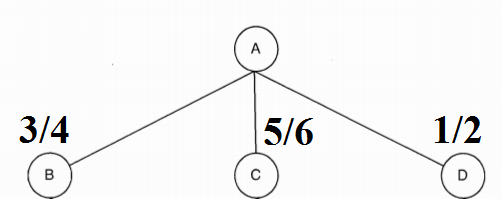
\includegraphics[scale=0.50]{1_Presentation/1.1_Our_project_Dan/tree}}
  \caption{An exploring tree :\newline The probabilities related to the nodes are the numbers, so the best node is the node B according to the statistics. See more in part 2.1.} %use \ref{nameOfSection} (and \label{nameOfSection})
  \centering
\end{figure}
The \emph{Monte Carlo Tree Search} has been used in the past for \textit{Draughts}, or \textit{Chess}. By exploring numerous random possibilities, it will be able to take good decisions in order to win a game of \emph{Arimaa}.
This algorithm will be parallelized in order to use it in a multi-core machine, improving its efficiency by allowing it to go deeper into the search tree.
\newline

Different parallelization methods will be considered, in order to choose the most adapted to this project.
%Thanks to the results of these latest methods, we will be able to choose a state resulting of the current move. Then we will explore the tree and with the same methods as before, we will figure out what the opponent will most probably do. The way we will be exploring the tree will only depend on the parallelization method. %Didn't understand a thing
The first part of this project will be the analysis of the latest papers concerning the technologies that might be of use.
The next part will consist in choosing among these technologies, in order to decide on the specifications.
\newline

Finally, in the last part, a solution will be implemented, and executed on Grid5000, a cluster of multi-core machines.
The interesting part about this project is the creation of an Artificial Intelligence as optimized as possible.


